
\documentclass{article}
\usepackage{graphicx}
\usepackage{outlines}
\usepackage{multirow}
\usepackage{tabularx}
\usepackage{wrapfig}
\setcounter{secnumdepth}{5}
\setcounter{tocdepth}{5}

\makeatletter
\renewcommand\paragraph{\@startsection{paragraph}{4}{\z@}%
  {-3.25ex\@plus -1ex \@minus -.2ex}%
  {1.5ex \@plus .2ex}%
  {\normalfont\normalsize\bfseries}}
\renewcommand\subparagraph{\@startsection{subparagraph}{5}{\z@}%
  {-3.25ex\@plus -1ex \@minus -.2ex}%
  {1.5ex \@plus .2ex}%
  {\normalfont\normalsize\bfseries}}
\makeatother


\begin{document}

\title{CyPhyML Language User Documentation}
\author{Institute for Software Integrated Systems (ISIS)\\Vanderbilt University}

\maketitle

\tableofcontents
\newpage

\section{Overview}
This document will help a user of the CyPhyML language.
\subsection{Modeling Activities}
The primary modeling activities are Component Models, Design Space, Designs, and Test Benches.

\subsection{A Picture, As A Figure, With Text Wrapping}
\begin{wrapfigure}{r}{0cm} % "placement and width parameter for the width of the image space.
\centering
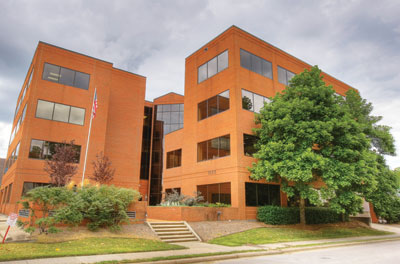
\includegraphics[scale=0.40]{eng-musicrow.jpg}
\caption{It's an image, ya'll.}
\label{imageyall}
\end{wrapfigure}
I hear the train a comin'. It's rollin' 'round the bend, and I ain't seen the sunshine since I don't know when. I'm stuck in Folsom Prison, and time keeps draggin' on. But that train keeps a-rollin', on down to San Antone.

When I was just a baby, my mama told me: "Son, always be a good boy. Don't ever play with guns."

\section{Aspects}
Many structures are common across all four modeling activities.
\subsection{ValueFlow}

The ValueFlow aspect is used in all four modeling activities, designs (Component Assemblies), Components, Design Space models (DesignContainers), and Test Benches. This aspect is used to express the static properties of a component or an assembly of components, and the relationships and dependencies between those values. By static, we mean that these values are set at design time, and do not change while the system is functioning. For example, the weight and length of an engine component are captured within the ValueFlow aspect. The ValueFlow aspect also captures the formulas needed to describe parametric components. For example, a driveshaft component design with parametric length will include a formula to describe its weight as a function of material density, diameter, and length. Formulas are evaluated at by an interpreter.

\subsubsection{Primary Concepts / Example}
Properties are represented by various types of value flow objects in the model. Value flow objects can be connected to each other representing assignment of the objects's numerical value from a source value flow object to a destination object. They also serve as inputs and outputs to formula objects via connections.

There are three main classes of value flow objects: Property, Parameter, and Metric. Since the three represent measurement of some physical quantity, they have a common attribute called Value that represents the current numerical value in addition to referencing a unit of measurement object in the model. Units of measurement are defined in a seperate aspect and will not be discussed here.

\begin{figure}
\centering
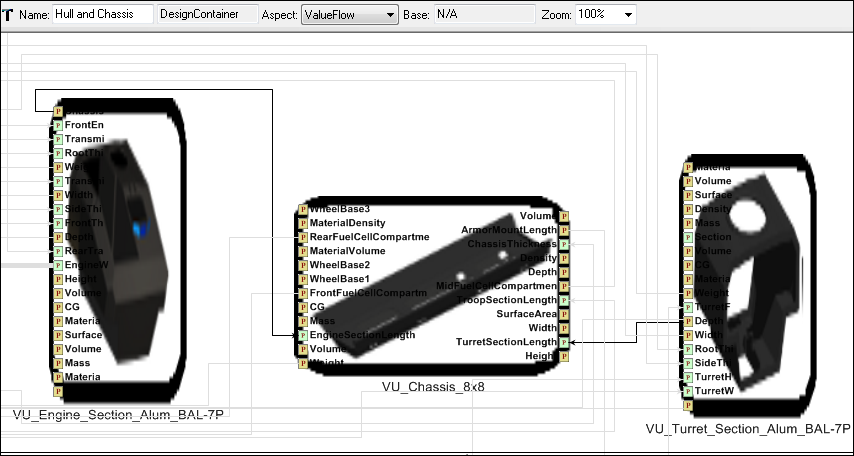
\includegraphics[scale=0.40]{Figures/cadParameter_VF.png}
\caption{Hull and Chassis Model.}
\label{fig:cadParameterVF}
\end{figure}
A Parameter object represents a static property of an object that can be tuned by a system designer at design-time. CADParameter is a specialization of Parameter. When a CAD model is built, the value of this object is used to set a specific parameter in the component's CAD representation. This is useful with parametrically-sizeable components, where the size of a component (or a feature of a component) depends on the size of another component that it is composed with. Figure \ref{fig:cadParameterVF} shows the Hull and Chassis portion of the IFV design space model. The VU\_Chassis\_8x8 component's TurretSectionLength and EngineSectionLength CADParameter objects get their Value attribute populated by VU\_Turret\_Section\_Alum\_BAL-7P's Depth Property object and VU\_Engine\_Section\_Alum\_BAL-7P's ChassisDepthMount Property object respectively.

\begin{figure}
\centering
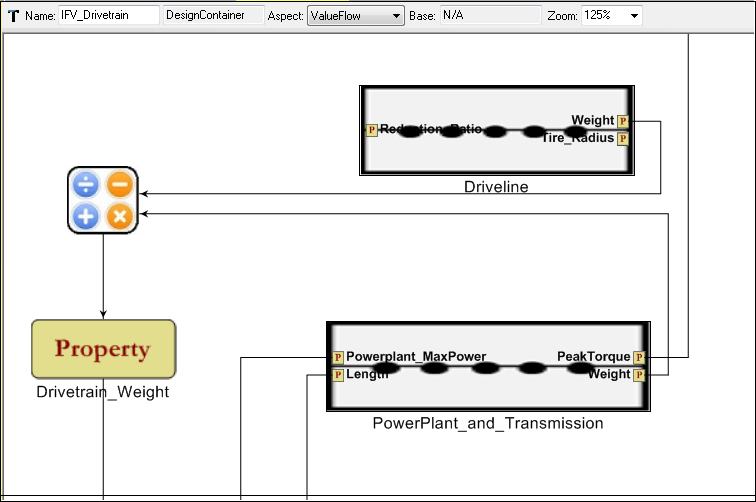
\includegraphics[scale=0.40]{Figures/Property_VF.png}
\caption{Drivetrain Design Space Model.}
\label{fig:propertyVF}
\end{figure}
A Property object represents a static property of an object or assembly. Properties of components cannot directly be changed at design time during design space model construction. Examples of Property are the weight of a damper and max power of a transfer case. Properties can be calculated from Parameters and other Properties using formula objects. Figure \ref{fig:propertyVF} shows the IFV\_Drivetrain design space model. In the figure, the Drivetrain\_Weight Property object is the sum of the Weight Property objects of Driveline and PowerPlant\_and\_Transmission. CADProperty is a specialization of Property. In practice, the value of a CADProperty must be calculated within a CAD tool, after which the result can be written back to the model. Examples of CADProperty in the current IFV model is the center of gravity and density of a Driver Hatch.

\begin{figure}[t]
\centering
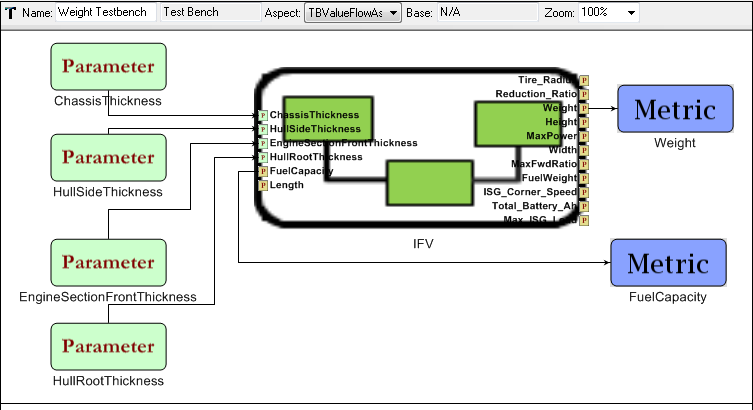
\includegraphics[scale=0.40]{Figures/Metric_VF.png}
\caption{Weight TestBench Model.}
\label{fig:metricVF}
\end{figure}
A Metric object is only used in test benches, test environments for testing composed systems, to capture outputs of running a test. A test bench is typically run on multiple designs of a system with the resulting metrics sometimes visualized in a GUI tool called Dashboard and compared across the designs. Figure \ref{fig:metricVF} shows the Weight TestBench model whose sole purpose is used for calculating the metric Weight and FuelCapacity of different IFV designs given an initial set of tunable input Parameter objects like HullSideThickness, ChassisThickness, etc.

\subsubsection{Using Formulas}
Formulas define relationship of connected value flow objects. There are two types of formulas in the CyPhy model used for describing calculation of property, parameter and metric quantities in the model. SimpleFormula are used for addition, multiplication, minimum, maximum, and geometric and arithmetic means. CustomFormula is a user defined algebraic expression using names of value flow objects or user define variable names. Incoming connections to a formula connects value flow objects  to the formula represents inputs used in the formula calculation. Outgoing connections represent output destinations to assign the calculated value to. A formula needs at least one input (incoming connection) and can be assigned to multiple value flow objects as well as other formulas.

A SimpleFormula has an attribute called Method which lets the user pick from the set of predefined mathematical functions to use on the input value flow objects. Addition, minmum, maximum, and average operations require that the units of input and output value flow objects be of the same dimension. If an input object doesn't not have an assigned unit, an attempt is made during evaluation process to automatically assign a compatible unit. For multiplication operations, the unit of inputs do not need to have the same dimesions. During evaluation process, the output's expected dimension is calculated based on the inputs' dimensions and checked against the actual dimension of the output's assigned unit. Figure \ref{fig:simpleformula} shows a SimpleFormula with inputs from Drivetrain, Hull and Chassis, and Turret assemblies and feeding the resulting sum to a Property object called Weight.
\begin{figure}[t]
\centering
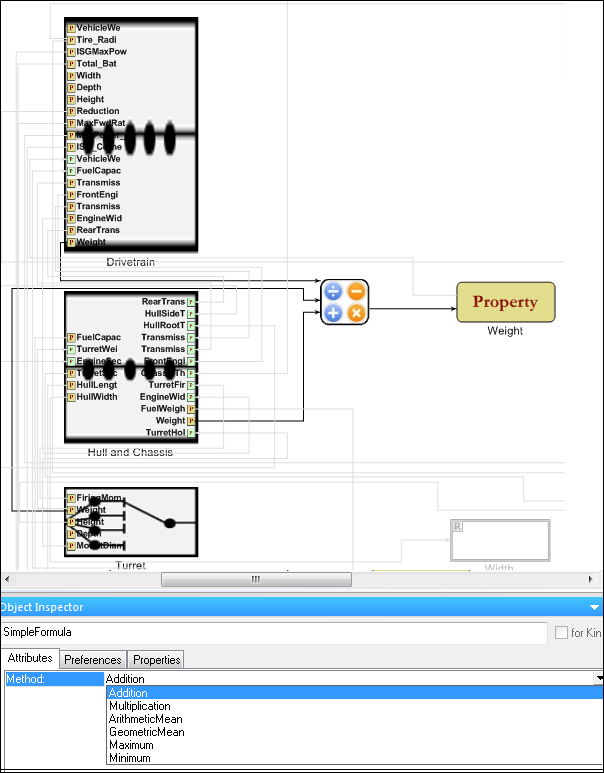
\includegraphics[scale=0.40]{Figures/simpleFormula_VF.png}
\caption{Simple Formula.}
\label{fig:simpleformula}
\end{figure}

A CustomFormula does not have any predefined operations. The user needs to type in a mathematical expression in the Expression attribute. During the evaluation process, third-party tool APIs (muParser) are called to parse and evaluate the expression. CustomFormulas are used primarily for surrogate equations in the IFV model. Units are not checked on CustomFormula intputs and outputs. The next subsection gives more detail on the syntax of CustomFormulas.

\paragraph{Formula Syntax}
CustomFormula supports algebraic expressions formed by combining constants, variables, mathematical operators and predefined functions. Variables can be the name of the input value flow object or the Variable Name attribute on the incoming value connection of a CustomFormula object. The supported operators and functions are listed in Tables \ref{tab:builtinfcntable} and \ref{tab:optable}. Built-in functions can support one more arguments, multiple arguments need to be seperated by commas and enclosed within a parenthesis. The arguments can be either constants or variables. The syntax for using an operator is (x operator y) where x and y are constants or variables.

\begin{table}
\parbox{.45\linewidth}
{
	\centering
	\begin{tabular}{ | l | l |}
	\hline
   Name & Num Argc \\ \hline    
    sin&1 \\ \hline
    cos&1 \\ \hline
    tan&1 \\ \hline
    asin&1 \\ \hline
    acos&1 \\ \hline
    atan&1 \\ \hline
    sinh&1 \\ \hline
    cosh&1 \\ \hline
    tanh&1 \\ \hline
    asinh&1 \\ \hline
    acosh&1 \\ \hline
    atanh&1 \\ \hline
    log2&1 \\ \hline
    log10&1 \\ \hline
    ln&1 \\ \hline
    exp&1 \\ \hline
    sqrt&1 \\ \hline
    sign&1 \\ \hline
    rint&1 \\ \hline
    abs&1 \\ \hline
    min&$>$1 \\ \hline
    max&$>$1 \\ \hline
    sum&$>$1 \\ \hline
    avg&$>$1 \\ \hline
   \end{tabular}
   \caption{Supported Functions}
   \label{tab:builtinfcntable}
   }
\hfill
\parbox{.45\linewidth}
{
	\centering
	\begin{tabular}{ | l | l |}
	\hline
    Name & Meaning \\ \hline    
    =&assignment \\ \hline
    \&\&&logical and \\ \hline
    ||&logical or \\ \hline
    <=&less or equal \\ \hline
    >=&greater or equal \\ \hline
    !=&not equal \\ \hline
    ==&equal \\ \hline
    >&greater than \\ \hline
    <&less than \\ \hline
    +&addition \\ \hline
    -&subtraction \\ \hline
    *&multiplication \\ \hline
    /&division \\ \hline
    $\wedge$&raise x to the power of y \\ \hline
  \end{tabular}
  \caption{Supported Operators}
  \label{tab:optable}
  }
\end{table}

Figure \ref{fig:customformula} shows two ways of writing a CustomFormula in the IFV\_DriveTrain design space model. The CustomFormula expression on the left used the name of input Property objects, Drivetrain\_Weight and PowerPlant\_MaxPower, along with constants. The example on the right used the VariableName attribute of the connections between CustomFormula and Drivetrain\_Weight and PowerPlant\_MaxPower Property objects. Notice that the attribute is displayed on both of the connections themselves. Both ways of writing the expression is valid and VariableName attribute should be used when there are multiple input value flow objects with the same name for a CustomFormula. 
\begin{figure}
\centering
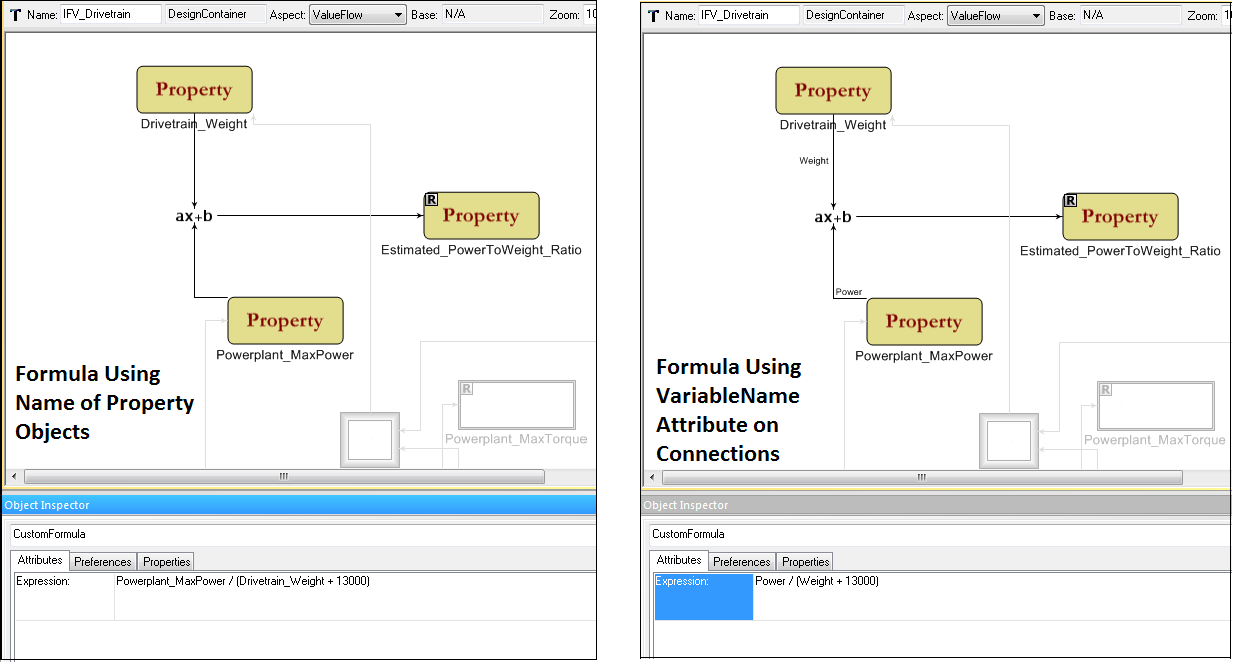
\includegraphics[scale=0.40]{Figures/customFormula_VF.png}
\caption{Custom Formula Using Name of Property Objects and VariableName Attribute on Connections.}
\label{fig:customformula}
\end{figure}



\subsection{Dynamics}

\subsubsection{Power Port Types}

\subsubsection{Composing Power Ports}

\paragraph{Modelica and BondGraph Power Port Differences}

\subsubsection{Composing Signal Ports}
\subsection{SolidModeling}

\subsubsection{First Section}
\paragraph{A Subsection}

\subsubsection{Second Section}


\section{Modeling Activities}
There are four primary modeling activities in CyPhyML.
\subsection{Component Models}
\subsubsection{Behavior Models}

\paragraph{Behavior Models in Components}

\subparagraph{Model Types}

\subparagraph{Port Mapping}

\subsubsection{CAD Models}
About CAD models in Component Models.

\paragraph{Linking Structural Interfaces to Datums}

\subsection{Design Models}
About Design Models.

\subsection{Design Space Models}
\label{sec:designspace}
Design Space Modeling is the central part of the Design Flow Process of Cyber-Physical Systems (CPS). The Design Flow Process in AVM META is truly challenging involving many diverse interactions (designed and accidental) among components, in different physical domains (mechanical, thermal, electromagnetic, electrical, hydraulic, etc.) and across the interface between computational and physical. Interactions can be expressed as dependencies at design time or as physical power flows and information flows at run time. If designers and their design process are not prepared to recognize and manage such interactions, developments can suffer lengthy design iterations, and, at worst, failure due to unintended interactions discovered late in the design cycle, at integration time. For this reason, it is absolutely critical to correctly model the Design Space, including not only the plethora of design choices available, but also complex platform constraints to ensure that the chosen designs satisfy the requirements of the design. These design constraints arise not only from interactions among the individual components, but also due to functional and practical requirements of the design. For example, a bigger transmission works only if a diesel engine with large enough torque is used, or the vehicle must be able to acceleration a 2 m/s2 on a 20-degree uphill. Such constraints are complex to represent and require support for complex mathematical functions in the constraint language. The CyPyML Design Space Modeling provides a collection of modeling methods and tools for exploration and visualization of designs and design spaces, solving complex design constraints, and effective management of the design spaces and designs.

\subsubsection{Syntax}

\begin{figure}[t]
\centering
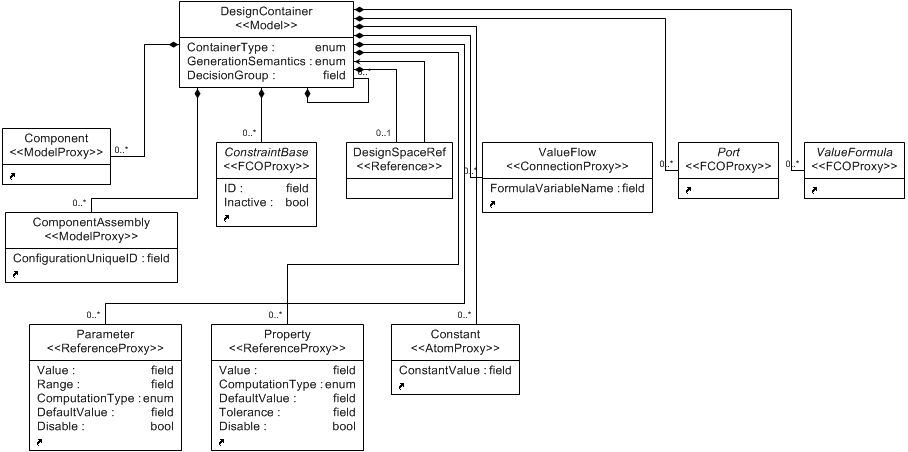
\includegraphics[scale=0.40]{Figures/DesignSpaceMetamodel.png}
\caption{Design Space Metamodel.}
\label{fig:designspacemetamodel}
\end{figure}

Figure \ref{fig:designspacemetamodel} shows the key modeling elements of CyPhyML pertaining to Design Space Modeling. As shown in the figure, the root element of the design space is of type DesignContainer. A DesignContainer can contain Components, Component Assemblies, Constraints, and DesignContainers. This allows to hierarchically model the Design Space mainly following the structural properties of the design. The enumeration shown for the DesignContainer's attribute ContainerType can have three possible values, viz. Compound, Alternative, or Optional. For a Compound DesignContainer, all its constituent elements must be selected as part of the design. Whereas, for an Alternative DesignContainer, only one among the choices available must be part of the design. The Optional DesignContainer contains only one DesignElement (a Component or a DesignContainer), which may or may not be part of the final design (i.e., optional containment).

\begin{figure}[t]
\centering
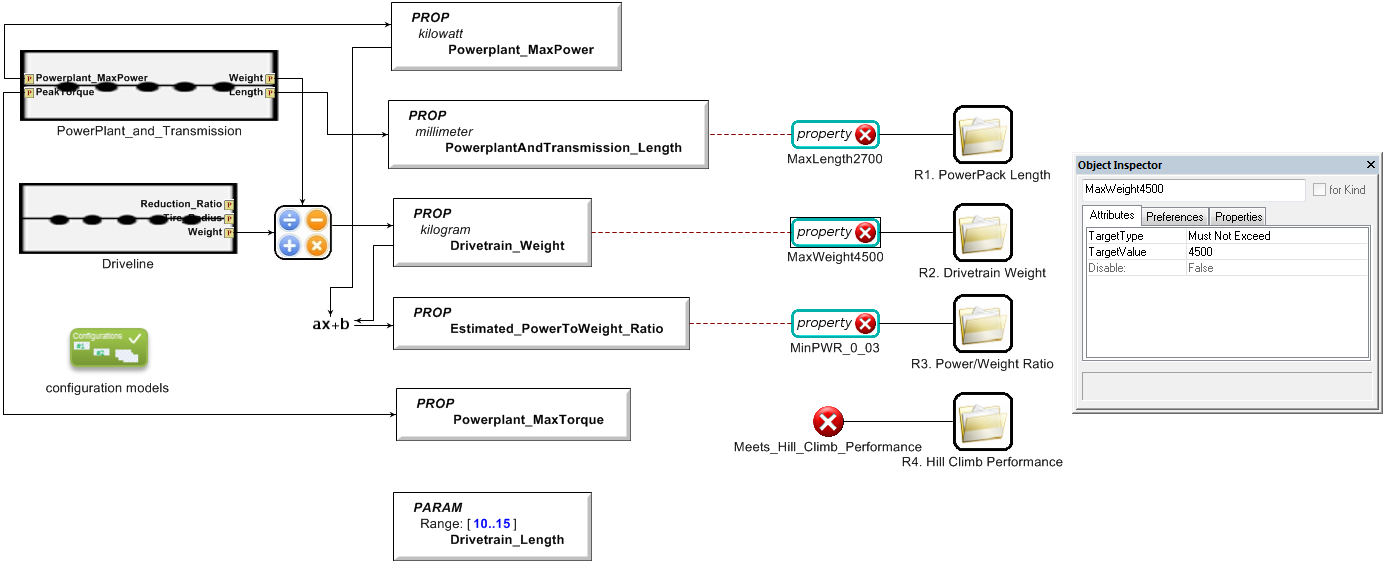
\includegraphics[scale=0.30]{Figures/IFVDrivetrainDesignSpace.png}
\caption{IFV Drivetrain Design Space Top-Level View.}
\label{fig:ifvdrivetraindesignspace}
\end{figure}

Figure \ref{fig:ifvdrivetraindesignspace} shows the top-level view of the IFV design space created using CyPhyML Design Space Modeling. The top-level design space itself is a Compound DesignContainer. In addition, it contains two child DesignContainers, viz. PowerPlant\_and\_Transmission and Driveline, both of which are Compound DesignContainers. The top-level DesignContainer also contains several design properties such as Powerplant\_MaxTorque and Drivetrain\_Weight. The properties of a DesignContainer may correspond to a basic property at that level in the DesignSpace or it may be a representative property that is calculated based on the chosen sub-elements of the DesignContainer. For example, the value of Drivetrain\_Weight property in a design will depend on which components were selected in that particular design. Design constraints can be applied on these properties. In addition to properties, CyPhyML also supports design parameters. Instead of taking a single value, design parameters can be used to specify a range of acceptable values for those parameters using the double-dot separator. The figure shows that the acceptable value of Drivetrain\_Length must be between 7-10 meters. The range can vary from -infinity to +infinity. Multiple ranges of parameters can be specified separated by a comma. These ranges specified for parameters are automatically translated into design constraints to ensure that the values of the parameters determined for acceptable designs are within acceptable ranges specified. Interested reader is referred to the secion on Property and Parameters for further information.

\begin{figure}[t]
\centering
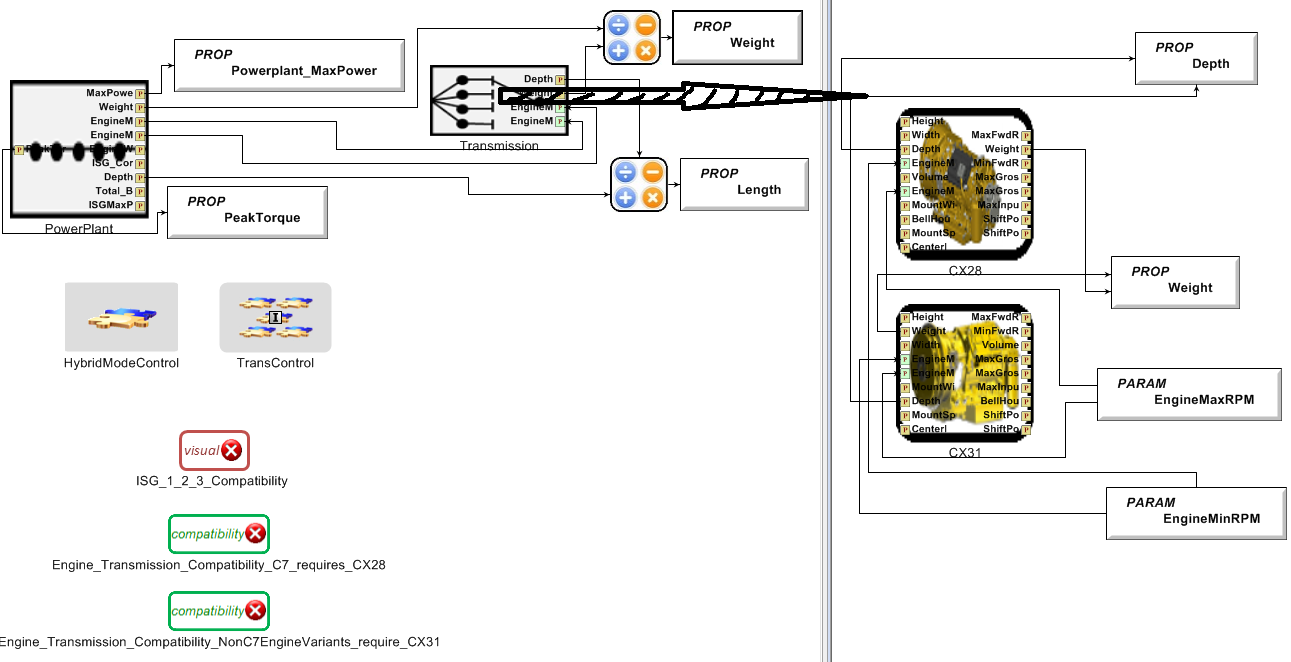
\includegraphics[scale=0.30]{Figures/AlternativeDesignContainer.png}
\caption{Alternative DesignContainer for Transmission and its Contents.}
\label{fig:alternativedesigncontainer}
\end{figure}


\paragraph{Alternative DesignContainers}

In the IFV drivetrain design space, the container PowerPlant\_and\_Transmission contains an Alternative DesignContainer for the transmission because two transmissions are available to choose for the design. Figure \ref{fig:alternativedesigncontainer} shows the Alternative DesignContainer for Transmission and shows its contents when expanded. As can be seen the IFV drivetrain has a choice of two transmissions, viz. CX28 and CX31.

\begin{figure}[t]
\centering
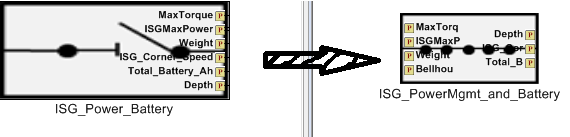
\includegraphics[scale=0.50]{Figures/OptionalDesignContainer.png}
\caption{ISG Power Battery Optional DesignContainer and its Contents.}
\label{fig:optionaldesigncontainer}
\end{figure}

\paragraph{Optional DesignContainers}

As show in Figure \ref{fig:optionaldesigncontainer}, in the IFV drivetrain design space, the container ISG\_Power\_Battery is an Optional DesignContainer. It contains only one DesignElement called ISG\_PowerMgmt\_and\_Battery. This means that in a IFV design ISG\_PowerMgmt\_and\_Battery may or may not be present (depending on whether the hybrid drivetrain control is used or not).

\paragraph{Constraints}
The feasible set of designs for a design space contains all possible combinations of the choices represented in the design space. This set contains an exponentially huge number of designs. However, not all designs are valid. To ensure that only meaningful and valid designs are selected, CyPhyML Design Space Modeling specification of several types of design and performance constraints. CyPhyML's DEsign Space ExploRaTion Tool (DESERT) ensures that only those designs are selected that satisfy the constraints modeled in the design space.

\subparagraph{PropertyConstraint}
Property constraints are the most basic type of constraints. It basically constrains the value of the associated property to be less than, less than or equal to, equal to, greater than or equal to, or greater than a specified value. In figure \ref{fig:ifvdrivetraindesignspace}, the property constraint is shown on IFV drivetrain maximum weight and ensures that the maximum drivetrain weight is less than or equal to 4500 Kgs.

\subparagraph{VisualConstraint}

\begin{figure}[t]
\centering
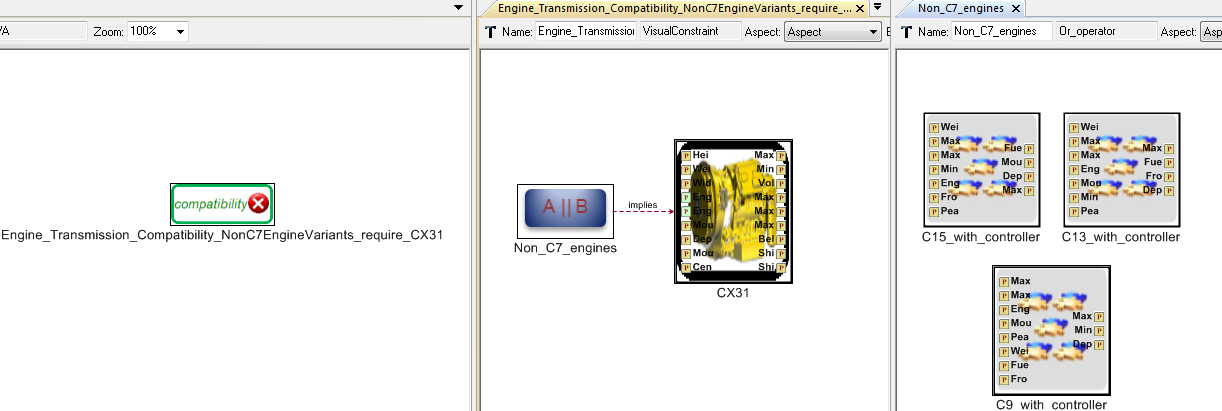
\includegraphics[scale=0.30]{Figures/DesignSpaceVisualConstraint.png}
\caption{Visual Constraint -- Engine\_Transmission\_Compatibility\_NonC7EngineVariants\_require\_CX31.}
\label{fig:designspacevisualconstraint}
\end{figure}

VisualConstrains are used to easily specify compatibility constraints in CyPhyML. In figure {fig:ifvdrivetraindesignspace}, several compatibility constraints are shown. One of them is Engine\_Transmission\_Compatibility\_NonC7EngineVariants\_require\_CX31. Figure \ref{fig:designspacevisualconstraint} shows the constraint fully expanded. Note that it uses an Or operator to combine variants of diesel engines that are not C7 and then uses an implies connection with the transmission CX31 to apply the compatibility constraint.

\begin{figure}[t]
\centering
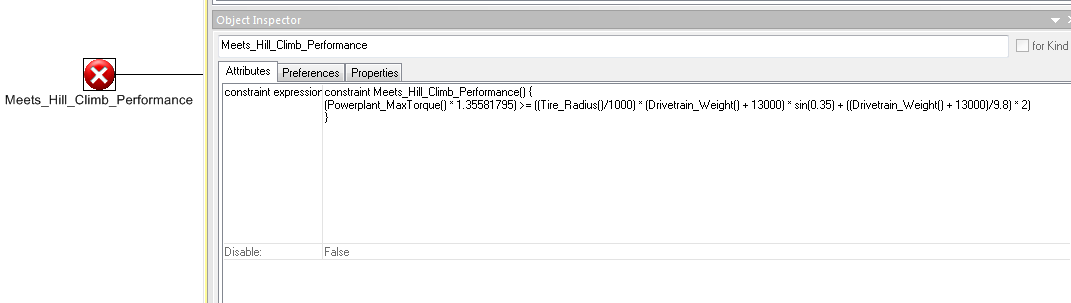
\includegraphics[scale=0.30]{Figures/DesignSpaceTextualOCLConstraint.png}
\caption{Example of manually written raw OCL-like CyPhyML design space constraint.}
\label{fig:designspacetextualoclconstraint}
\end{figure}

\subparagraph{Constraint Language}
All constraints in CyPhyML Design Space modeling are converted into raw OCL form. Although graphical means such as property constraints, parameter ranges, and visual constraints are sufficient to specify all types of constraints supported in CyPhyML, user can still choose to write them in textual OCL format, if needed. As an example, the constraint Meets\_Hill\_Climb\_Performance in figure \ref{fig:ifvdrivetraindesignspace} is a manually written constraint in raw OCL-like form. This is further shown in figure \ref{fig:designspacetextualoclconstraint}.

\subparagraph{DecisionGroup}

In the design space example above, the Driveline DesignContainer inside IFV drivetrain contains 8 HalfShaft\_and\_WheelAssembly DesignContainers. Each of these 8 DesignContainers are Altenative DesignContainers and contain choices of 3 different types of wheels. This leads to a total 3**8 = 6561 combinations just for choosing the wheels. However, in any IFV design, all wheels should be of same type. So, in reality there are only 3 choices. To represent that we can add several Visual constraints to make sure that if one type of wheel is chosen for any container, then same wheel type is chosen for all other 7 containers. However, this is highly cumbersome. CyPhyML provides an easier way to co-relate this same decisions of different Alternative DesignContainers by means of DecisionGroups. A DecisionGroup contains references of Alternative containers that essentially belong to the same decision of the choice that needs to be made. CyPhyML's DESERT solver recognizes DecisionGroups and automatically ensures that in any design same DesignElement is chosen for all Alternative DesignContainers that are part of the same DecisionGroup.

\subsubsection{Executing, Exporting, and Refinement}

Once the Design Space has been modeled along with all the compatibility, correctness, and performance constraints, the next step involves invoking the DESERT tool to generate configurations (point designs) that satisfy all the design space constraints. User is referred here to the DesignSpaceHelper tool document for further information (DesignSpaceHelper.docx). The configurations generated are lightweight such that they only contain references of the components chosen and no hierarchy or connections. These design can be converted into fully-specified designs with hierarchy and connections by using CyPhyML's tool called CyPhyCAExporter. User is referred to document CyPhyCAExporter\_OneSheet.docx for further information about it. One of the critical requirements of Design Space exploration and configuration generation is the capability to perform coarse-grained exploration and constraint satisfaction on some parts of the design space and when satisfactory configurations have been generated, do deeper refinement of those parts on the selected results. Such a capability is provided by CyPhy design refinement tool. User is referred to the document CyPhyDSRefiner..docx for further information on CyPhyML's design space refinemnet tool. CyPhyML also provides a tool called CyPhyDSEConverter. This tool allows the user to convert existing components, component assemblies, or design containers into a new design container that can now include new parts in it for design extentions and exploration of that particular child design space part of the original design space. User is referred to the document CyPhyDSEConverter.docx for more information on it. Lastly, CyPhyML also provides a tool to assist the user in determining the usefulness of refining a particular component, component assembly, or a design container. This tool is called CyPhyCriticalityMeter. CyPhyCriticalityMeter goes through all design spaces in the model and generates valid design configurations for them in memory and assigns a number to each DesignElement to specify how many configurations that DesignElement was chosen in and out of how many total configurations. User is referred to the document CyPhyCriticalityMeter.docx for more information on it.

\subsection{Test Benches}
\subsubsection{Core Concepts}
About core TestBench concepts.

\paragraph{System Under Test}
\subparagraph{Test Injection Point}
\paragraph{Parameters}
\paragraph{Metrics}
\paragraph{Dashboard}
\paragraph{PCC Features}
\subsubsection{Static Test Benches}
About Static Test Benches.
\subsubsection{Dynamics Test Benches}
About Dynamics Test Bench.

\paragraph{Constructing / Syntax}

\paragraph{Executing}
\subsubsection{CAD / FEA Test Benches}
The currently supported CAD TestBench model is used to perform a static structural finite element analysis (FEA) on a subset of components from a design space model (see section \ref{sec:designspace}). FEA involves automatically creating an assembly of components of interest, creating a FEA deck consisting of a 3D mesh with load and constraint information, then submitting the deck to a FEA solver to generate results. Results are post-processed via scripts to compute structural metrics. In a test bench model, the user can choose the metric(s) of interest for each component. The currently supported metrics for a structural analysis include:	
\begin{itemize}
\item Factor of Safety
\item Maximum VonMises Stress
\item	Maximum Shear Stress
\item Maximum Bearing Stress
\end{itemize}
Support is currently being added to compute a Quality Rating for the above stress metrics.

\paragraph{Constructing / Syntax}
A CAD TestBench model contains references called TestInjectionPoints that refer to components from a design. The user would include only the components from the design space model for the subsystem that he/she would like to analyze as TestInjectionPoints. Some IFV components are parametric, meaning their CAD models have attributes that need to be specified at runtime during the creation of the assembly for analysis. These attributes appear as CADParameter objects in a component's model in the ValueFlow Aspect and are computed by another interpreter before running FEA. The TopLevelSystemUnderTest object determines the starting point for computing value flow parameters and properties including CADParameters. This typically points to the top most design container in a design space model.

A component surface or a portion of a surface is defined by a group of datum points on the component that form an area that would be constrained or acted upon by a load. The datum points are depicted as ports on the TestInjectionPoint in the test bench model. In the generated 3D mesh, any mesh grid points that fall within the defined area would be constrained or acted upon by a load. To create a surface in the model, the user would connect a Surface object to AnalysisPoint datum ports on a TestInjectionPoint when in Connect Mode in GME. The surface types provided by the modeling language are:  
\begin{itemize} 
\item Circle - Requires three datum points as follows:
		\begin{itemize} 
		\item Point at the center of the circle
		\item Point on the circumference of the circle
		\item Point defining the plane of the circle.  This point would typically (but not necessarily) be on the circumference of the circle; however, it cannot be collinear with the line formed by the first and second points. 
	\end{itemize}
\item Concentric Circles � Two concentric circles defined by three datum points as follows: 
		\begin{itemize} 
		\item Point at the center of the circle
		\item Point on the circumference of the outer circle
		\item Point on the circumference of the inner circle.  Because this point also defines the plane of the circles, it cannot be collinear with the line formed by the first and second points. 
		\end{itemize}
\item Cylinder - Requires 3 datum points as follows: 
		\begin{itemize} 
		\item Point defining the start of the cylinder centerline (i.e. axis)
		\item Point defining the end of the cylinder centerline
		\item Point at a distance from the centerline that equals the cylinder radius.  This point would typically (but not necessarily) be on the cylinder surface.  If it is not on the cylinder surface, it would be offset from the beginning or end of the cylinder.  In any case, the distance between this point and a line defines the radius, where the line is a theoretically infinite line that is coincident with the centerline. 
		\end{itemize}
\item Polygon - Requires at least 3 ordered datum points.  The datum points must be ordered because the order defines the lines segments forming the polygon.  For example, points 1, 2, 3, and 4 would define a polygon with line segments 1-2, 2-3, 3-4, and 4-1.  Noticed that the closing of the polygon by line segment 4-1 is implied.  Repeating 1 at the end (e.g. 1, 2, 3, 4, 1) would be erroneous.      
\item Sphere - Requires 2 datum points as follows:
		\begin{itemize} 
		\item Point at the center of the sphere
		\item Point on the circumference of the sphere
		\end{itemize}
\end{itemize}

 
Loads distort the physical structure thereby creating stress. The CAD TestBench modeling language provides Acceleration (gravity), Force, and Pressure loads. Acceleration is not applied to a single component but to the entire assembly formed by composing TestInjectionPoints. Acceleration is defined by magnitudes in the x, y, z directions. Force load has a Force and a Moment component defined by forces in the x, y, and z directions and moments about the x, y, and z axes. Pressure load is defined by a magnitude value. To apply Force and Pressure loads to a Surface object in the model, the user would connect the Load object to a Surface object when in Connect Mode in GME. Acceleration load is simply placed in the test bench model since it's applied to the composed assembly. A single load object can be connected to multiple Surface objects.

Boundary conditions are used to constrain portions of the model to remain fixed or to be displaced by a prescribed amount. In static structural analysis, boundary conditions are typically used to prevent parts from moving as a rigid body. Boundary conditions provided in the language are: Ball, Displacement, and Pin constraints. Displacement constraint has a Rotation and a Translation component in the x, y, and z direction either as fixed, free or a scalar value. Displacement can only be applied to a Polygonal surface. Pin constraint is defined by a free or fixed AxialRotation and AxialDisplacement attributes and can only be applied to a Cylindrical surface. Ball constraint can only be used on a Spherical surface.  Pin and Ball constraints are currently not supported. To apply constraints to a Surface object in the model, the user would connect a Constraint object to a Surface object when in Connect Mode in GME.

There are three types of Structural Metric objects available in the language: StressMetric, FactorOfSafety, and MaximumDisplacement. The StressMetric has a Type attribute which the user can set to either Mises, Shear, or Bearing. The Type attribute determines which stress types appear in the resulting log and Dashboard XML file after post-processing analysis results. A StressMetric object should be connected to TestInjectionPoint(s) of interest.  The stress metric is only computed for the connected TestInjectionPoint(s).

\begin{figure}[t]
\centering
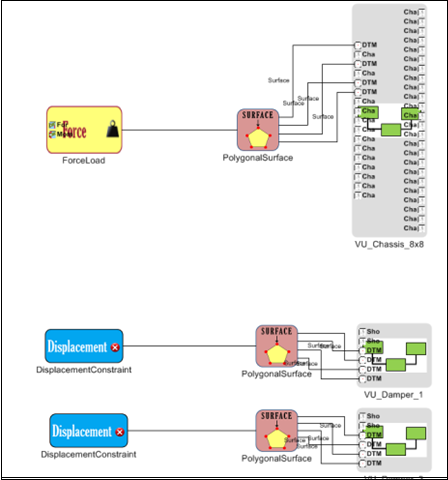
\includegraphics[scale=0.40]{Figures/chassisDamper_cadTB.png}
\caption{Chassis Damper Cad Test Bench.}
\label{fig:chassis_damper}
\end{figure}

Figure \ref{fig:chassis_damper} shows portions of the Chassis Damper CAD TestBench model in the current IFV model. This test bench is used to analyze a single chassis along with eight connecting dampers to compute stress distributions under a set of loads and constraints. There are nine TestInjectionPoints, one for chassis and eight for the eight dampers. There is a single Force load on the chassis with a scalar value in the y direction on the Force component. All eight of the dampers have a displacement constraint with rotation in the y direction set to free and all other attributes set to fixed. Only polygonal surfaces are used for the loads and constraints and they are connected to datums in each component. The connections themselves are annotated with Surface to indicate the location. Similarly, when other types of Surface objects are connected to datum points the connection would be annotated to show the point's location on a Surface object.

\paragraph{Executing}
\begin{figure}[t]
\centering
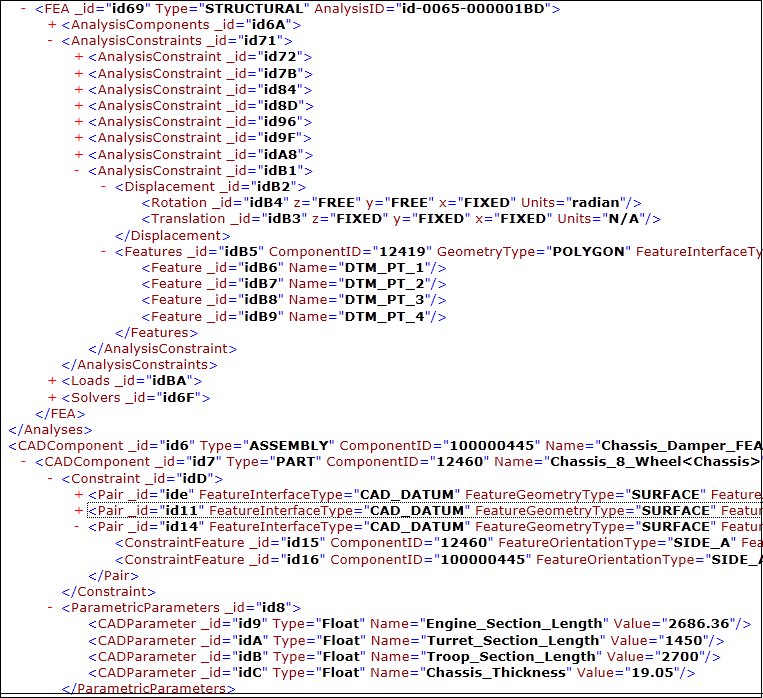
\includegraphics[scale=0.40]{Figures/xmlOut_cadTB.png}
\caption{XML file generated from CyPhy2CAD with assembly information and FEA load and constraints.}
\label{fig:cadTB_xml}
\end{figure}
The CyPhy2CAD interpreter processes a test bench model and produces an XML file containing the assembly definition.  The assembly definition specifies how components are constrained to one another via datums, and it specifies the FEA loads and constraints.  Figure \ref{fig:cadTB_xml} shows the generated XML file. The interpreter requires 2 directories, one for storing the generated files and a second one for the location of Creo part files.

\begin{figure}[t]
\centering
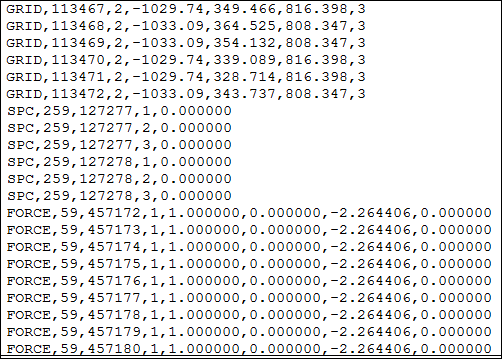
\includegraphics[width=0.5\textwidth]{Figures/inpDeck_cadTB.png}
\caption{XML file generated from CyPhy2CAD with assembly information and FEA load and constraints.}
\label{fig:inpDeck_cadTB}
\end{figure}
A program called CADCreoParametricCreateAssembly is invoked that calls Creo SDK APIs to automatically build a Creo assembly based on the xml file as well as calling Creo's mesher to generate a 3D mesh of the assembly in the form of a Nastran input deck, see figure \ref{fig:inpDeck_cadTB} for a section of the deck. In the figure, GRID keyword is followed by coordinates of grid points in the mesh, SPC keyword corresponds to constraints from the model applied to mesh grid points, and lines with FORCE keyword are Force loads on grid points. A bat file calls a FEA solver passing in the Nastran input deck as the argument. Currently we are using Abaqus from SIMULIA as our solver and are working on supporting more solvers. Abaqus returns several files, but the main one we post-process is a binary data file (*.odb file). The post-processing step involves computing the maximum stresses (VonMises, Shear, and Bearing) and factory of safety based on the maximum stresses and material properties for component(s). PNG files showing stress gradients across component(s) in 7 views (iso, top, bottom, left, right, back, and front), VRML, and 3D Xml files are also generated. 3D XML file contains 3D data that can be opened in a player to view stress gradients and animated deformations. A log file is generated that contains status and error messages as well as metric information for debugging purposes. An XML file conforming to Dashboard schema is generated so that the metrics can be visualized in the Dashboard.

Figure \ref{fig:isogradient} shows the output stress gradient png file in the iso view. Notice that high stress areas are marked by red and low stress area by blue.

\begin{figure}
\centering
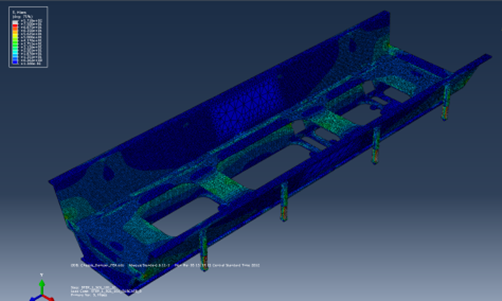
\includegraphics[scale=0.40]{Figures/iso_gradient_cadTB.png}
\caption{ISO view of stress gradient in Chassis.}
\label{fig:isogradient}
\end{figure}

\end{document}